\section{The sweep engine}

Full-wave azimuth sweeps are driven by
\cmd{sim/pipeline/sweep\_runner.py}, exposed in the GUI's FW sweep
tab. A sweep rotates the specimen through a set of azimuths and runs
the solver at each, exactly as the machine rotates the disk under its
probe. Sessions are resumable by construction: each sweep directory
under \cmd{out/sweeps/} holds a \cmd{config.json} and one trace
archive per completed azimuth, so an interrupted campaign continues
where it stopped, and the analysis layer reads completed azimuths
without waiting for the rest.

Each azimuth's traces are stored raw. Everything derived (envelopes,
picks, fits, backprojections) is recomputed downstream, so a stored
sweep never bakes in an analysis decision.
Figure~\ref{fig:trace} shows the anatomy of one stored trace.

\begin{figure}[htb]
  \centering
  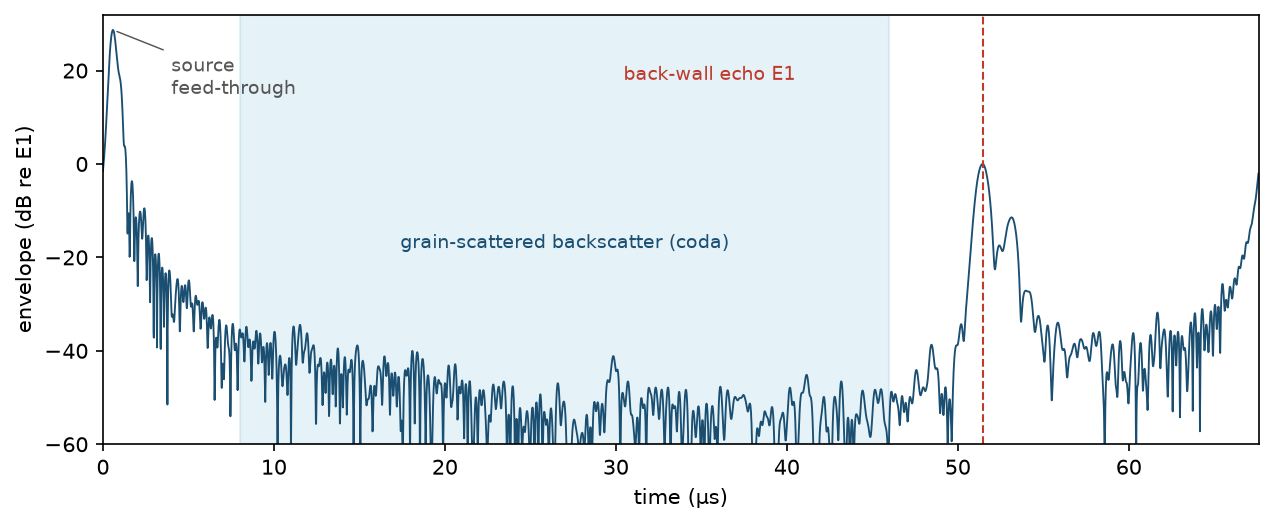
\includegraphics[width=0.95\textwidth]{figures/trace-anatomy.png}
  \caption{A clean 2 MHz reference trace (aligned fabric, envelope in
    dB relative to E1): source feed-through, the grain-scattered
    backscatter that fills the record, and the back-wall echo E1 near
    52 microseconds whose time of flight carries the velocity
    observable.}
  \label{fig:trace}
\end{figure} The arc backprojection
view (\cmd{sim/pipeline/}) maps coherent energy in the received
traces back into the disk and is the quickest qualitative check that
a sweep contains structure rather than noise.
